\chapter{Contributions}

In the following sections, we present the main contributions related to the \framework~framework and the Homogeneous Graphs Benchmark.

\section{Overall Architecture}

Figure \ref{fig:architecture} depicts the frameworks and the main components belonging them, additionally, it also denotes that which components are reused from Train Benchmark.

\begin{figure}[!ht]
	\centering
	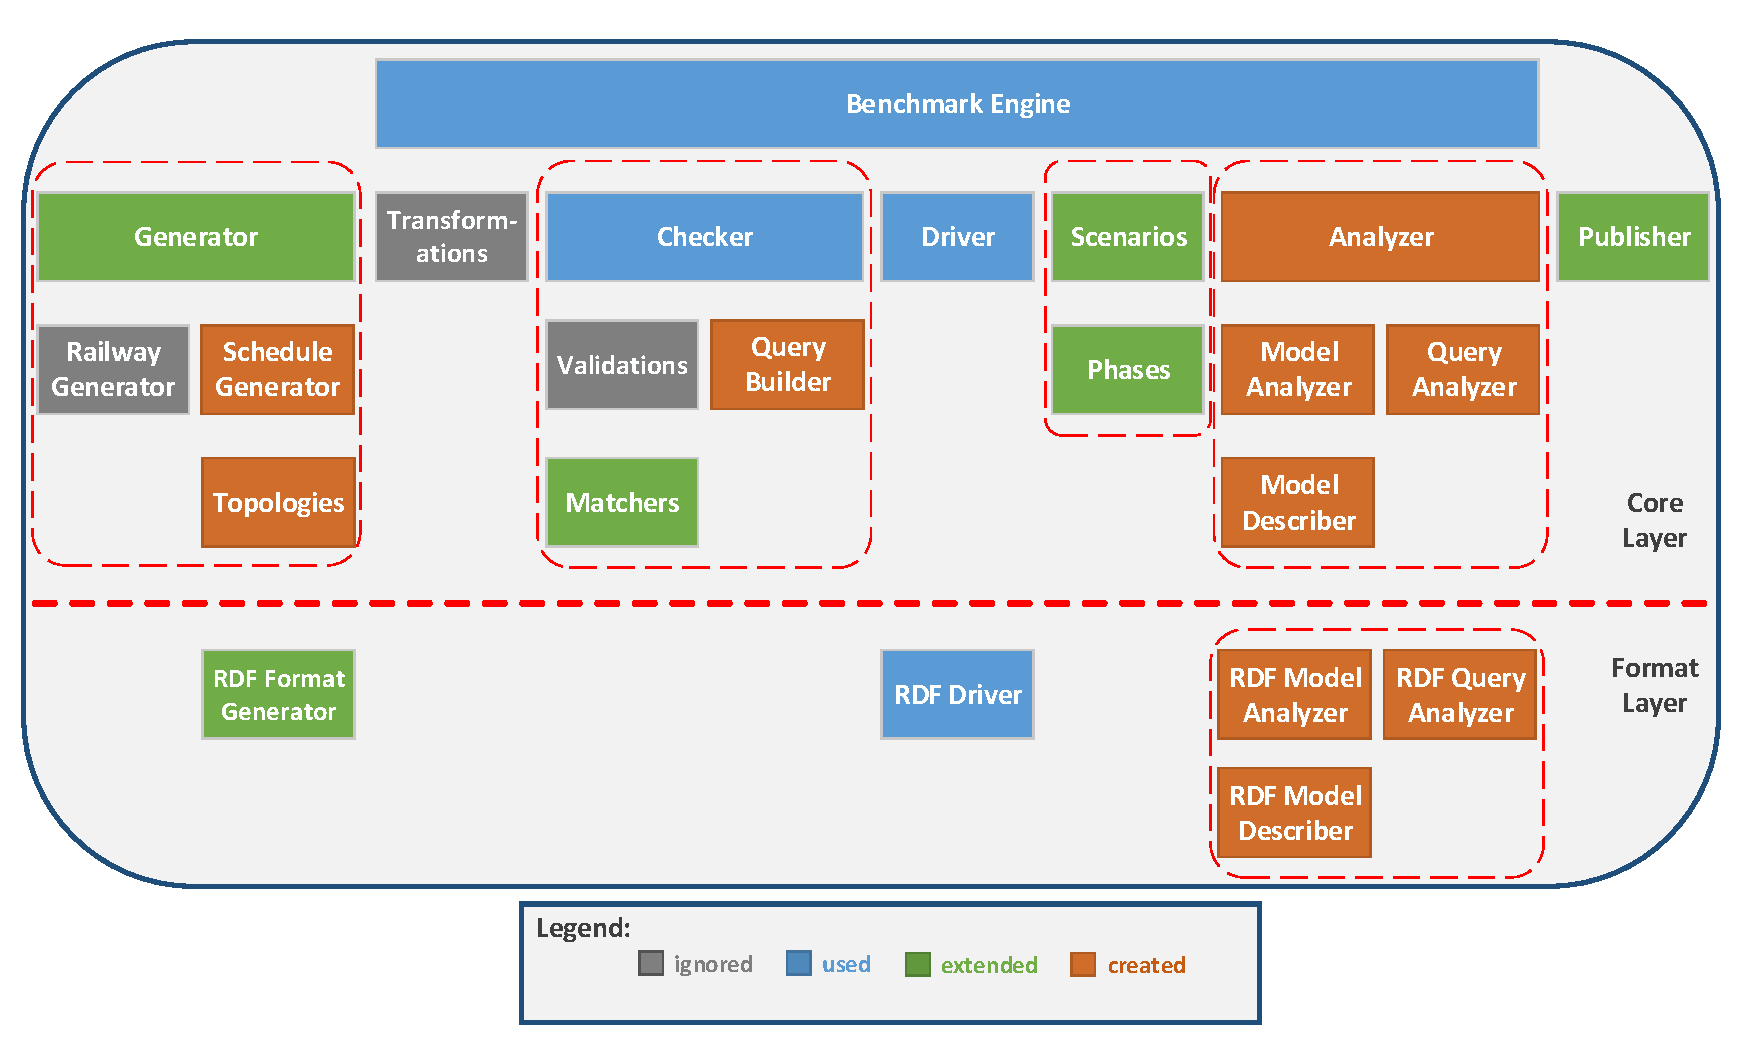
\includegraphics[width=150mm, keepaspectratio]{figures/architecture.pdf}
	\caption{The architecture of our approach.}
	\label{fig:architecture}
\end{figure}

In the following parts, we introduce the components.

\paragraph{Benchmark Engine}
The \textsf{Benchmark Engine} in MONDO-SAM is responsible for evaluating an arbitrary sequence of phases consecutively. A phase is considered as the atomic execution unit in a benchmark. The engine also measures the evaluation times of phases, hence, it is the component that measures the performance of query evaluations in our work.

\paragraph{Analyzer Components}

The \textsf{Model} and \textsf{Query Analyzer} units belong to the \framework~framework and define an interface for the metrics calculation. The \textsf{Model Analyzer} investigates the model related metrics, and the \textsf{Query Analyzer} relates to the query definitions. As it can be observed, the concrete metric calculations---\textsf{RDF Model Analyzer} and \textsf{RDF Query Analyzer}---appear in the HG Benchmark.

\paragraph{Metrics}

The definitions of metrics---such as \textsf{Model Metrics}  and \textsf{Query Metrics}---can be found in \framework. The model metrics symbolize graph metrics with applying the commonly used naming conventions from graph theory. Note that the HG Benchmark does not contain further RDF-based metrics implying that we use the graph-based naming conventions in our work.\\
The query metrics connect to the definitions of the queries, and they do not relate to the query performance or the result set of the evaluations.

\paragraph{Generators}

The generator components belong to the HG Benchmark. The abstract \textsf{Generator} unit is utilized from Train Benchmark. The \textsf{Stations Generator} component is responsible for transforming the real-life British Railway Stations model to RDF. Last, the \textsf{Topology Generators} construct different homogeneous graphs fitting to well-known topologies and transform them to RDF format.

\paragraph{RDF Driver}
The \textsf{RDF Driver} manages the connections between the measured RDF databases and the benchmark framework, furthermore, it also accomplishes the loading of the models. 

\paragraph{Query Executor and Query Builder}

The query evaluations are achieved by the \textsf{Query Executor} component. The \textsf{Query Builder} is responsible for creating and altering the query definitions in runtime.

\section{British Railway Stations}

In order to test our regression models on an entirely different graph, we introduce a real-life model to our work. We use a model of train stations provided by the \textit{Network Rail} company that runs, maintains, and develops Britain's rail tracks~\cite{network_rail}. Network Rail publishes a number of different data available to developers, one of them is a \textit{daily extracts and updates of train schedules}~\cite{schedules_data} that we intend to use.

The data contains approximately 10 000 British stations that belong to train schedules as destinations. We concentrate on the network of stations, and map it to a graph where every vertex symbolizes a station. An edge is drawn between two nodes---so two stations---if these stations appear consecutively in a destinations path belonging to a schedule.

\section{Uniform Model Generation}

It is an essential expectation from the HG Benchmark to guarantee uniform model generation among the topologies indicating the same size of the generated models. We propose a model generation technique to generate topologies with the same amount of nodes and edges.

\subsection{Number of Nodes}

The random graph and the Watts-Strogatz model are constructed by initializing $|V| = N$ number of vertices, and then the algorithms determine which one of them become adjacent. In the scale-free model generator, the nodes are created incrementally until $|V| = N$. As a conclusion, a precise number of nodes can be obtained regarding these topologies.

The only one problem about generating topologies with a certain number of nodes is the recursive algorithm of the hierarchical graph, which algorithm has to be terminated.

\subsubsection{The Termination of the Hierarchical Network Algorithm}\label{sec:hierarcical_contribution}

Since the generation of hierarchical network is recursive instead of being incremental---as in the case of the three other topologies---it is inevitable to determine a termination from the recursion. The termination point is evident, as soon as the number of created nodes reaches the limit, the algorithm has to be stopped. However, it cannot be predicted in which phase the algorithm stops exactly. As a consequence, the possible failures have to be managed.

\begin{figure}[!ht]
	\centering
	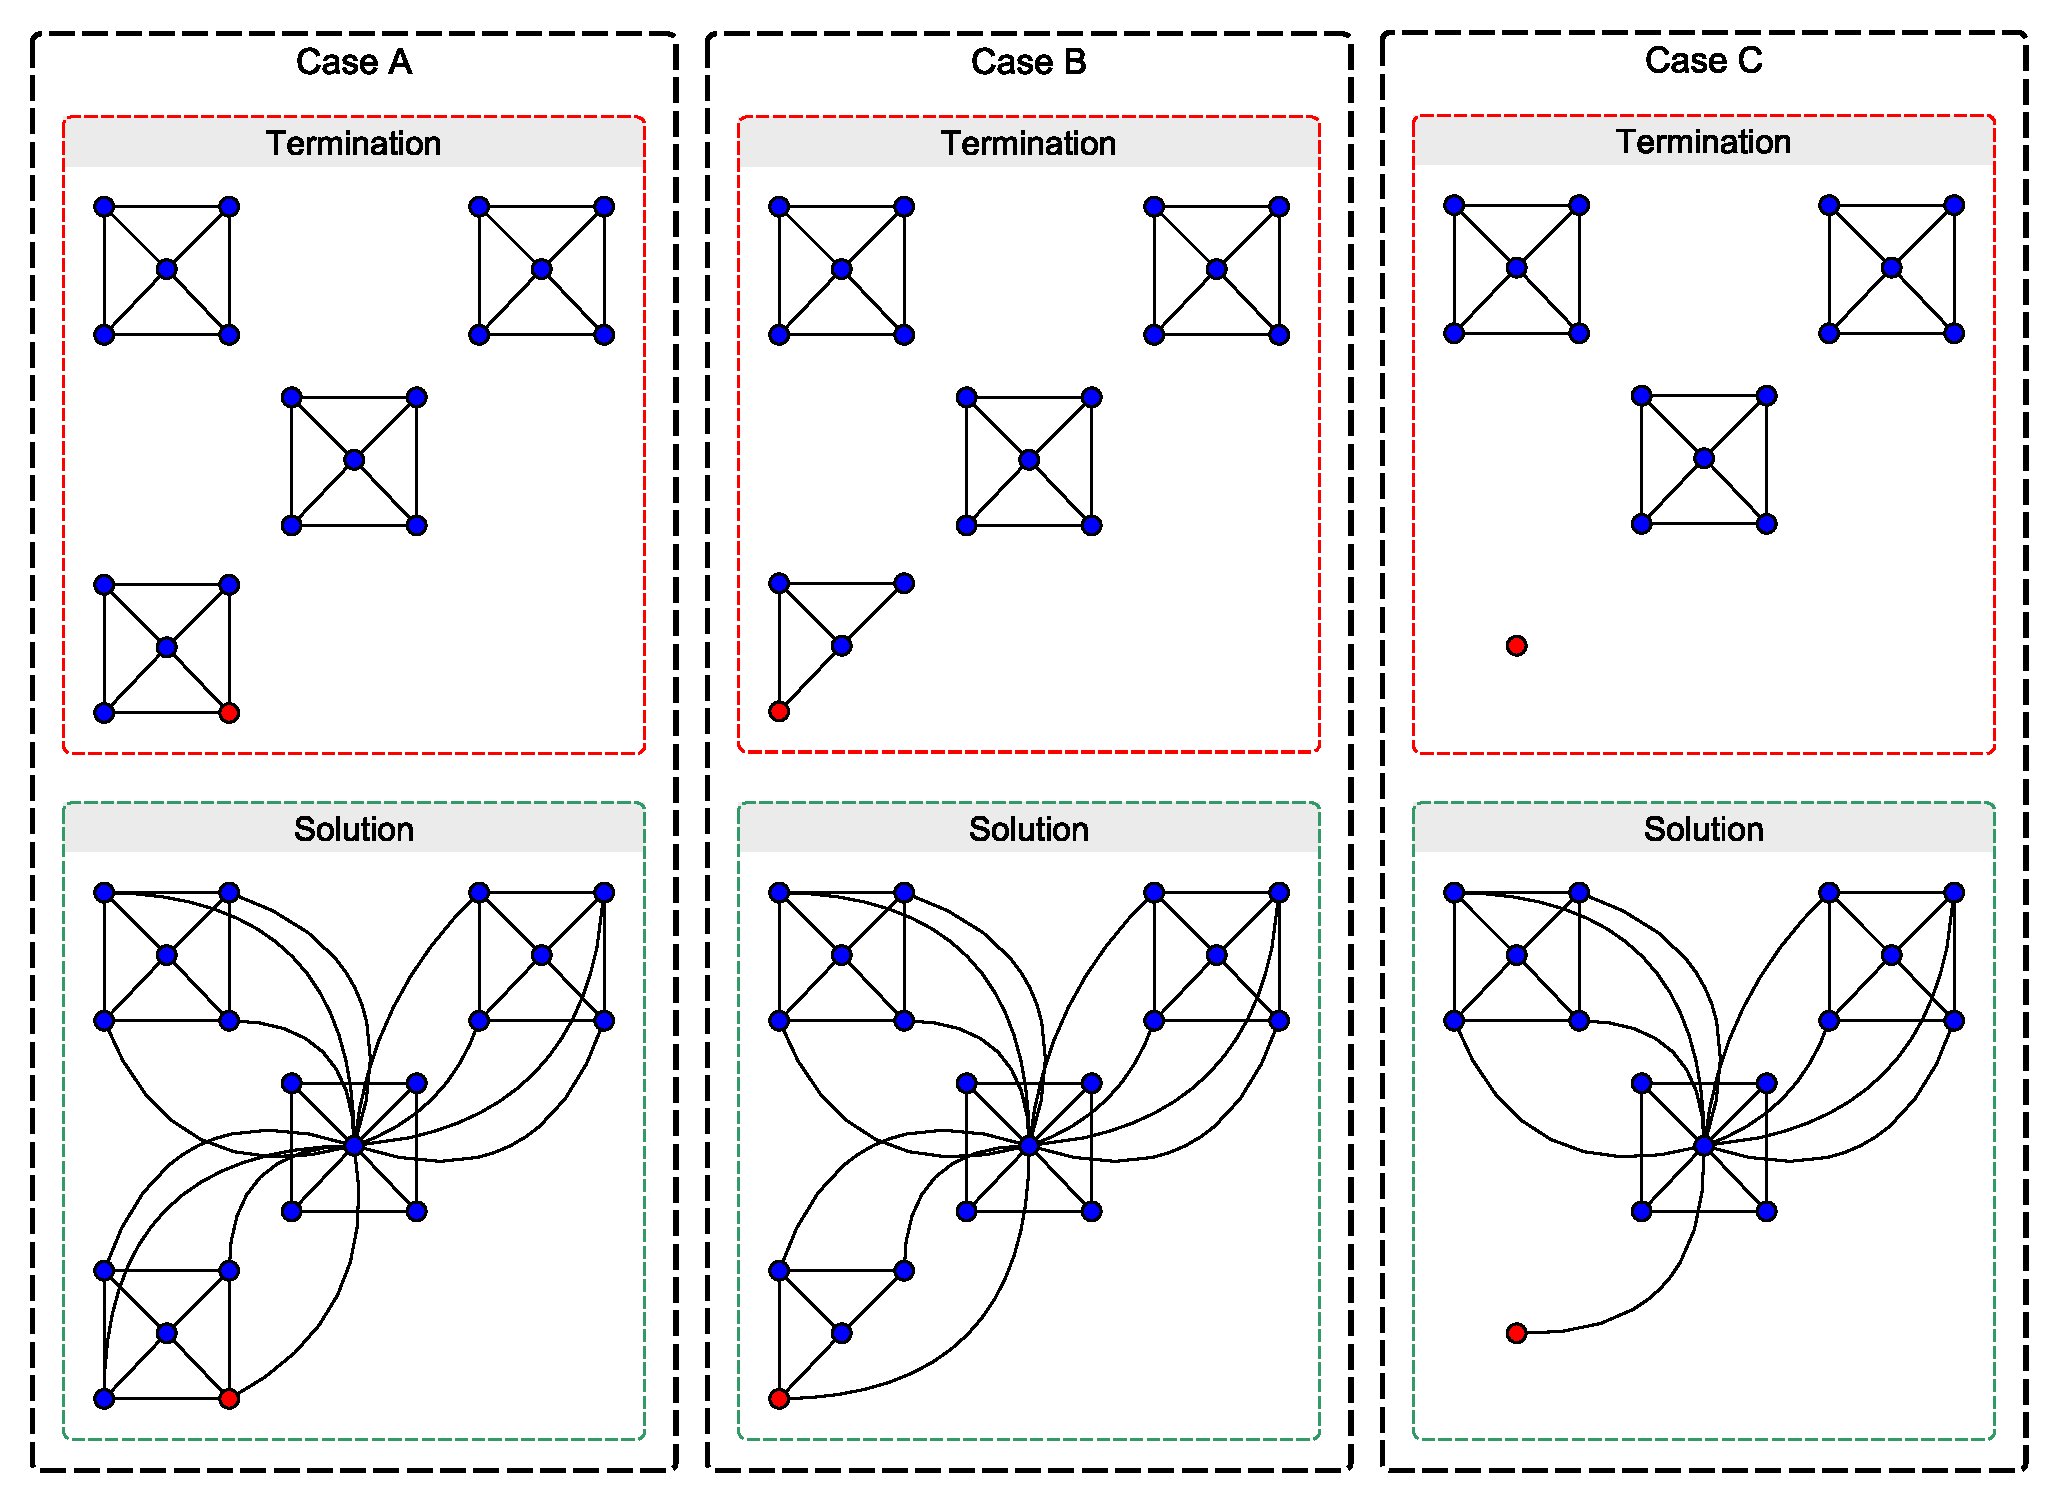
\includegraphics[width=150mm, keepaspectratio]{figures/hierarchical.pdf}
	\caption{Possible termination problems in the hierarchical graph generation}
	\label{fig:hierarchical_problems}
\end{figure}

The possible problematic cases are demonstrated in Figure \ref{fig:hierarchical_problems}. In \textsf{Case A}, \textsf{B}, and \textsf{C}, the expected numbers of nodes are 20, 19, and 16, respectively. As it can be observed in these cases, this limit is always reached before the fourth cloning occurs, since 5 clusters should be created with 25 vertices at the end of this step in the recursion.

In the solution in \textsf{Case A}, the generator stops the clone procedure and connects the diagonals to the center. Regarding \textsf{B}, the termination happens during the generation of a cluster. As a solution, the last cluster becomes partial, and similarly, every diagonal is attached to the center. \textsf{Case C} represents that scenario when the last cluster only consists of one node. To prevent isolation, the last vertex is considered as a diagonal, and be connected to the center.

\subsection{Number of Edges}

%todo note that the diagonal nodes are also connected — links not visible on hierarchical graph
In terms of the random graph, scale-free, and WS model, their generation algorithms can be adjusted arbitrarily, meaning that an optional number of nodes or edges can be achieved. Actually, reaching a certain amount of nodes or edges in these networks are handled separately.

Unfortunately, the creation of nodes and edges in the hierarchical graph occurs together. Since the amount of edges depends on the number of nodes and iterations in the recursive algorithm, it cannot be configured arbitrarily. A solution is that we adjust the other topologies to have the same number of edges as the hierarchical model. This solution requires to calculate the exact number of edges in a hierarchical network with respect to the iteration.

\subsubsection{Estimate the Number of Edges in Hierarchical Graphs}

The literature relating to hierarchical graphs does not mention the exact number of edges or its correlation to the amount of nodes, hence, we propose a solution to estimate $|E|$ in the recursive algorithm for every iteration.

At first, let define the necessary variables hereunder:
\begin{itemize}
	\item{$i$}: Represents the current iteration in the original hierarchical algorithm.
	\item{$c$}: Indicates the number of clones in every iteration.
	\item{$n$}: The cluster size is denoted by $n$, which cluster is a $K_n$ complete graph. %todo cluster from nothing?
	\item{$F_i$}: It indicates the constructed graph after the $i$ iteration. %todo why F? maybe change it to H later
	\item{$|E_{F_i}|$}: The number of edges of $F_i$.
\end{itemize}

In the 0. iteration, the hierarchical graph consists of one $K_n$ cluster. Formally defining, $F_0 = K_n$, and $|E_{F_0}| = |E_{K_n}| = \frac{n \cdot (n-1)}{2}$. In the 1. iteration, the algorithm clones $F_0$ for $c$ times, and connects the peripheral nodes from each $F_0$ to the center node. It entails that 
\begin{align}\label{eq:f1_version1}
	|E_{F_1}| = (c+1) \cdot |E_{K_n}| + c \cdot (n - 1)	
\end{align}
since $c+1$ number of $K_n$ can be found in $F_1$, and $c \cdot (n - 1)$ edges can be drawn from the $c$ number of replicas to the center.

Note that in the first iteration $K_n$ can be substituted with $F_0$, and the algorithm in the first part of the $i$ iteration creates $c$ number of replicas of the result of the $i-1$ iteration, namely, $F_{i-1}$. In the second part of the $i$ iteration, the algorithm connects the clusters from the cloned replicas to the center node. These connections are made between the peripheral nodes in each replica and the center, which indicates that the algorithm---in the $i$ iteration---connects $n-1$ peripheral nodes from $c$ number of replicas of $F_{i-1}$, and due to $F_{i-1}$ includes $c^{i-1}$ number of clusters, we obtain

\begin{align}\label{eq:fi_formula}
	|E_{F_i}| = (c+1) \cdot |E_{F_{i-1}}| + c \cdot c^{i-1} \cdot (n - 1)	= (c+1) \cdot |E_{F_{i-1}}| + c^i \cdot (n - 1)
\end{align}

We are not finished yet, since Equation \ref{eq:fi_formula} is equal to the number of edges of a completely finished hierarchical network. However, the generation algorithm in \framework~is possibly terminated to reach a certain number of nodes, which leads to the fact that $|E_{F_i}|$ must be scaled down by the proportion of the maximum ($|V_{F_i}|$) and the required number ($|V_H|$) of vertices. If the hierarchical graph we intend to generate is denoted by $H$, then
\begin{align}\label{eq:h_formula}
	|E_H| = |E_{F_i}| \cdot \frac{|V_H|}{|V_{F_i}|}
\end{align}
where $\frac{|V_H|}{|V_{F_i}|} \leq 1$.

By using Equation \ref{eq:h_formula}, we can calculate the number of edges of a hierarchical graph and configure the other topologies to reach the same quantity.

\subsubsection{Configure Random Graph}
From the two known algorithms, Gilbert's $G(n,p)$ model is adapted to the framework, which implies that the exact value of $p$ has to be determined from the number of edges in the hierarchical graph, $|E_H|$. Based on~\cite{random_p}, the $p$ probability can be calculated from the number of nodes and edges as follows:
\begin{align}
	p = \frac{|E_H|}{\binom{|V|}{2}}
\end{align}
where $|V|$ denotes the number of nodes.

\subsubsection{Configure Watts-Strogatz Model}\label{sec:watts_generation}

Regarding the Watts-Strogatz model, in the beginning of the generation algorithm, $K$ number of consecutive nodes are connected to each other. During the algorithm, by rewiring the edges the amount of $|E|$ is not changed. As a conclusion, in order to achieve a uniform size similarly to the hierarchical graph, $K$ has to be adjusted as $K = \frac{|E_H|}{|V|}$.

Generally, the $K$ value in the algorithm is a constant integer. In order to configure the WS model properly, we extend the algorithm by defining an inclusive lower ($K_1$) and upper ($K_2$) bound for $K$, as $K\in[K_1, K_2]$, and we also assign a $p$ probability to $K$ that determines the likelihood of $K$ is equal to $K_2$ and $1-p$ to $K_1$. Derived from the equation $K = \frac{|E_H|}{|V|}$, it results in $K_1 = \Big\lfloor\frac{|E_H|}{|V|}\Big\rfloor$ and $K_2 = \Big\lceil\frac{|E_H|}{|V|}\Big\rceil$, additionally, the $p$ probability equals to the fractional part, as $p = \Big\{\frac{|E_H|}{|V|}\Big\}$. Hence, by turning $K$ to a random variable, we can generate WS models with the same number of edges as $|E_H|$.

\subsubsection{Configure Scale-Free Model}

The scale-free topology is generated incrementally, since every step a new node is inserted to the graph with $m$ number of new connections. To obtain $|E_H|$, the $m$ variable has to be configured. This leads to $m = \frac{|E_H|}{|V|}$.

In the original generation algorithm, every new vertex connects to a constant number of disjunct nodes, which indicates that $m$ is a constant integer. Similarly to the notion in the Watts-Strogatz model generation (\ref{sec:watts_generation}), this constant value is converted to a random variable based on a particular probability, derived from $|E_H|$.

\subsection{Possible Model Configuration}

In the artificially generated models the size, topology and density is optionally configurable. 

The size of the model---the number of nodes---is calculated by a formula as $|V| = s \cdot 2^i$, where $s$ is the step size constant and $i$ is a positive integer. It implies that an arbitrary model size can be obtained among the topologies.

Besides the size, the density of the graphs is also configurable, so the number of edges in the topologies. Since the hierarchical network is considered as the reference model due to the uniform model generation, the density parameter calibrates the generation algorithm of the hierarchical graph, namely, the size of the $K_n$ clusters with altering $n$. 

\section{Performance Analysis}

\subsection{Workflow}

A workflow in the HG Benchmark is divided into phases that are considered as the atomic execution units. An arbitrary sequence can be created among the phases, which---during the benchmark---are executed consecutively by the evaluation engine in MONDO-SAM.

\begin{figure}[!ht]
	\centering
	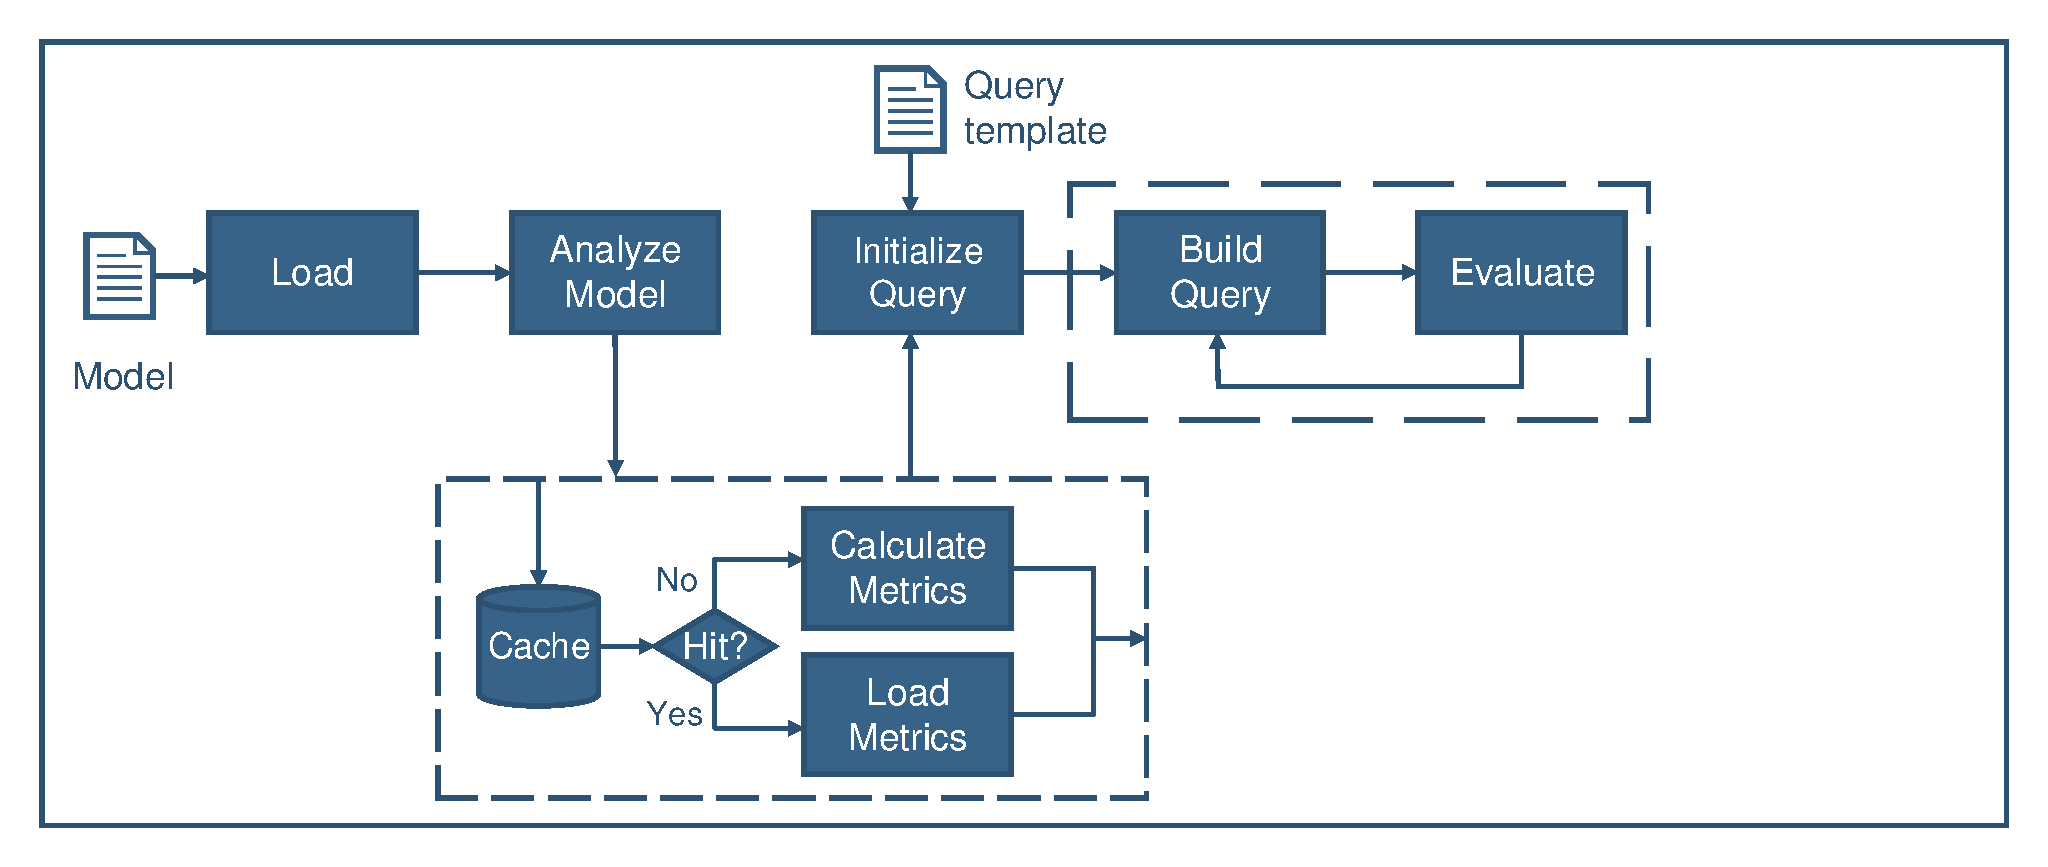
\includegraphics[width=150mm, keepaspectratio]{figures/workflow.pdf}
	\caption{The workflow of the HG Benchmark.}
	\label{fig:mondo_map_workflow}
\end{figure}

The workflow of the HG Benchmark is represented in Figure \ref{fig:mondo_map_workflow}. After loading the model, the framework calculates the model related metrics. Due to the fact that in the current phase of our research we do not consider model transformations, therefore, a particular model's metrics can be calculated only once in the beginning of the workflow, and more importantly, different runs of the benchmark can utilize the previously calculated metrics that belong to the same model. As it can be observed in the model analysis phase, the solution is achieved by using a cache for the calculated metrics and reusing its content if possible.

The features in the \textsf{Initialize} and \textsf{Build Query} phases are strongly correlated. These two phases entail the creation of dynamic queries. The first one provides a default query definition that can be parameterized, and the second phase assembles a complete query for the evaluation, as it injects parameters or alters the entire syntax. The latter operation implies that entirely different queries can be executed in a sequence.

Last, the evaluation phase is responsible for executing the query. The building and evaluating phases can be repeated implicating that more then one query can be evaluated in a sequence, even with different definitions.

\subsection{Metrics Calculation}
As we already emphasized, the \framework framework proposes two types of metrics. The first is the set of model descriptive metrics and the second relates to the query syntaxes. In the following, we introduce them and their calculations in the HG Benchmark.

\subsubsection{Model Metrics}
The model-based metrics are connected to graph metrics which appear in their naming conventions as well. Since we are concentrating on RDF tools in our work, we also define the corresponding interpretations. The metrics are listed hereunder.
%todo rdf and graph metrics
\begin{enumerate}
	\item{\textbf{Nodes:}} the number of nodes in the graph. In RDF, this equals to the number of unique subject and object values.
	\item{\textbf{Edges:}} the number of edges in the graph. Regarding RDF, this is equal to the number of predicates\footnote{With the consideration of \textsf{rdf:type} predicates, the number of edges metric represents the number of triples.} in the data.
	\item{\textbf{Maximum Degree:}} the maximum number of predicates per subjects.
	\item{\textbf{Average Degree:}} it is determined by calculating the degree of every existing node.
	\item{\textbf{Average Degree Distribution:}} denotes the probability that a randomly selected node’s degree is equal to the average degree.
	\item{\textbf{Higher Degree Distribution:}} the cumulative distribution of those nodes that have higher degrees than the average.
	\item{\textbf{Average Clustering Coefficient:}} this metric implies the calculation of clustering coefficient per every node.
	\item{\textbf{Average Shortest Path Length:}} the calculation of this metric requires the most cost, hence, the framework searches a limited number (100) of shortest paths between randomly chosen vertices and calculates the average length of them.
	\item{\textbf{Maximum Betweenness Centrality:}} the value of this metric is determined by the shortest paths. We count the occurrences of every intermediate node in the paths---which is the betweenness centrality of the vertices---and normalize the values to the $[0,1]$ interval by dividing them with the number of visited nodes. Since the value of betweenness centrality is individual per nodes, we use the maximum of them.
\end{enumerate}

\subsection{Queries}

We investigate the performance of two queries in our HG Benchmark. The first one relates to the concept of shortest path, and the second connects to the notion to investigate the spread of information in the graphs.

\subsubsection{Shortest Path Query}

The SPARQL definition of the query is shown below:\\
\lstinputlisting{content/queries/transitive.sparql}

The query uses the \textsf{*} operator from SPARQL Property Paths~\cite{property_path} in the \textsf{(base:neighbor)*} predicate which means an arbitrary length of path with the \textsf{neighbor} predicates. The query is considered as a parameterized query in which we inject two random identifiers instead the \textsf{ID} parameters. Finally, the query searches a path between those two randomly chosen nodes.

\subsubsection{Information Spread Query}
%todo mention spread of information in background betweenness
The query investigates the spread of information in the graph---by starting from a randomly chosen node---and it traverses the graph via the \textsf{neighbor} predicates to a three-hop distance. The concept of information spreading means that how fast the information can be forwarded among the nodes in the graph, or in other words, how many vertices can be reached from a certain node.\\
The SPARQL definition of the query is showed below. As it can observed, in every new navigation we filter the previously found nodes to prevent the traversal of the same nodes again.

\lstinputlisting{content/queries/spread.sparql}

\subsection{Tools}

We concentrate on RDF tools in our work which are listed in Table \ref{tab:tools}. The last two columns illustrate whether the execution of our defined queries is feasible in the particular tool or not. As the table suggests, the first query cannot be evaluated in \textsf{4store}, since it does not support the usage of property paths.

\begin{table}[ht]
	\footnotesize
	\centering
	
	\begin{tabular}{ l c c c c c}
		\toprule
		Name & Programming Language& Version & Query 1 & Query 2\\ 
		\midrule 
		AllegroGraph~\cite{allegro} & C, \CC & 5.0.0  & \textbullet&  \textbullet \\ \hline
		Blazegraph~\cite{blaze} & Java  & 1.5.2 & \textbullet & \textbullet\\ \hline
		4store~\cite{4store} & C  & 1.1.5 & & \textbullet \\ \hline
		Jena TDB~\cite{jena_tdb} & Java & 2.13.0 & \textbullet & \textbullet\\ \hline
		Sesame~\cite{sesame} & Java & 2.7.9 & \textbullet & \textbullet\\ \hline
		\bottomrule
	\end{tabular}
	\caption{The implemented tools in Train Benchmark}
	\label{tab:tools}
\end{table}


\subsection{Regression Analysis}

\subsubsection{MARS}


